% !TeX spellcheck = ru_RU
\documentclass{resume}

\begin{document}

%\fontfamily{ppl}\selectfont

\noindent
\begin{tabularx}{\linewidth}{@{}m{0.8\textwidth} m{0.2\textwidth}@{}}
{
    \Large{\textbf{Шипилов Фома}} \newline
    \small{
        \clink{
            \href{mailto:foma@shipilov.ru}{foma@shipilov.ru}
            \textbf{·} 
            \href{https://t.me/foma2u}{@foma2u}
        } \newline
        РФ, г. Москва
    }
} & 
{
    \hfill
    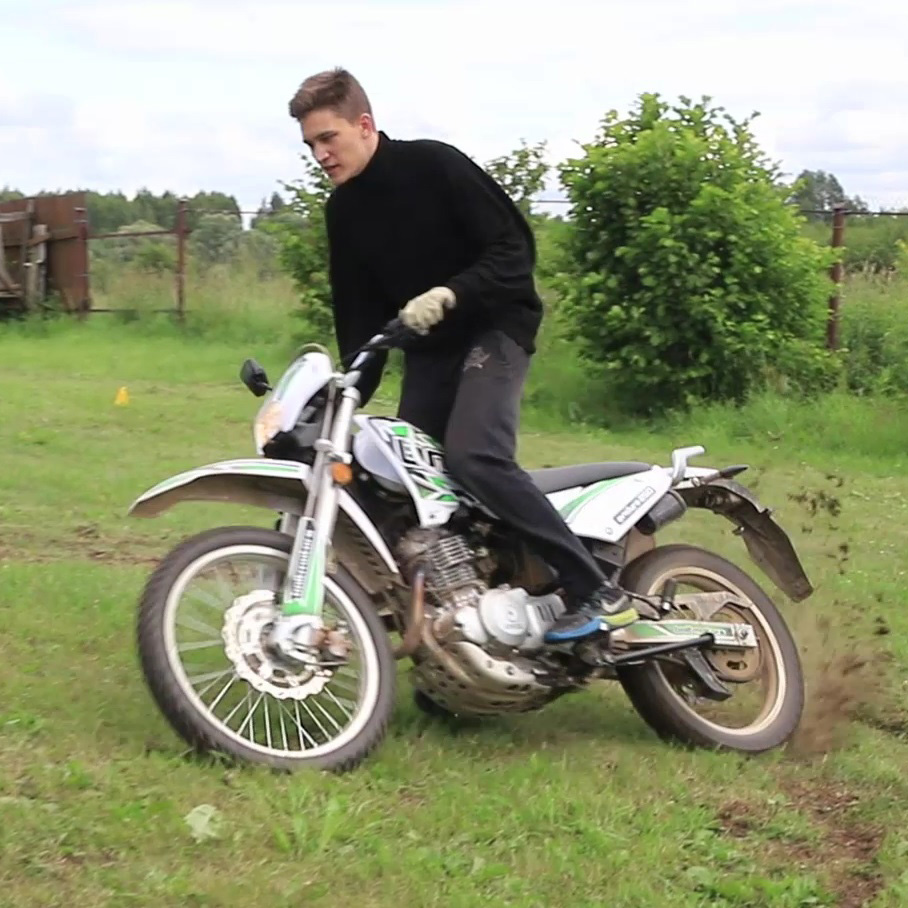
\includegraphics[width=2.8cm]{images/gr.jpg}
}
\end{tabularx}
\begin{center}
\begin{tabularx}{\linewidth}{@{}*{2}{X}@{}}
% left side %
{
    \csection{ОПЫТ РАБОТЫ}{\small
        \begin{itemize}
            \item \frcontent{Huawei}{Ассистент-инженер, Noah’s Ark lab\vspace{0.2em}}{-- Улучшение качества аниме с помощью ГАНов;\newline
            -- Разработка нелинейной сверточной модели деградации реальных изображений.}{Ноябрь 2020 -- Сентябрь 2021}
            \item \frcontent{ВШЭ}{Стажер-исследователь, Институт Искусственного Интеллекта (LAMBDA)}{-- Применение машинного обучения для быстрой реконструкции и симуляции аэрогелевых детекторов.\newline 
            \href{http://doi.org/10.1134/S106377882305037X}{What Machine Learning Can Do for Focusing Aerogel Detectors, Physics of Atomic Nuclei 86, 864 (2023)}}{С ноября 2021}
            \item \frcontent{ВШЭ}{Учебный ассистент, Факультет компьютерных наук}{Семинарист по Глубинному обучению 1}{2020 -- 2024, С сентября 2023}
        \end{itemize}
    }
    \csection{ОБРАЗОВАНИЕ}{\small
        \begin{itemize}
            \item \frcontent{Магистратура Data Science (англ.)}{ВШЭ, Сколтех (Программа двух дипломов MML)}{}{Студент}
            \item \frcontent{Трек магистратура-аспирантура}{ВШЭ}{}{Студент}
            \item \frcontent{Бакалавр 01.03.02 ПМИ}{ВШЭ}{}{2023, Диплом с отличием}
        \end{itemize}
    }
    \csection{ПРОЕКТЫ}{\small
        \begin{itemize}
            \item \frcontent{HiFi-GAN \clink{\href{https://github.com/xiyori/hw4_nv}{[github.com]}}}{Реализация модели HiFi-GAN из NeurIPS 2020}{}{PyTorch}
            \item \frcontent{secHNet \clink{\href{https://github.com/xiyori/secHNet}{[github.com]}}}{PyTorch на Haskell с нуля}{}{Haskell, C}
            % \item \frcontent{Visual Turing \clink{\href{https://github.com/xiyori/turing_machine_emulator}{[github.com]}}}{Turing machine IDE in \textit{C++}}{}{}
            \vspace*{-3em}
        \end{itemize}
    }
} 
% end left side %
& 
% right side %
{
    \csection{НАВЫКИ}{\small
        \begin{itemize}
            \item \textbf{Машинное обучение, анализ данных} \newline
            {\footnotesize -- Компьютерное зрение, сверх-разрешение, ГАНы, диффузионные модели, LLM, глубинное обучение в звуке, байесовские методы, линейная связность нейросетей\newline
            -- PyTorch, scikit-learn, OpenCV, NumPy, JAX, PySpark, Hadoop, Vowpal Wabbit}
            \item \textbf{Программирование} \newline
            {\footnotesize Python, C, C++, C\#, Haskell, x86/ARM Assembly, HTML/CSS, ReactJS, Lua}
            \item \textbf{CI/CD, другое} \newline
            {\footnotesize Docker, WandB, GitHub Actions, QuickCheck, GDB, Arch Linux, Shell}
        \end{itemize}
    }
	\csection{НАГРАДЫ}{\small
		\begin{itemize}
            \item \frcontent{Стипендия Яндекса}{ВШЭ}{Лауреат}{2022}
			\item \frcontent{Высшая лига, ПМИ}{ВШЭ}{Дипломы I и III степени}{2021, 2022}
			\item \frcontent{Я профессионал, математика}{Яндекс}{Призер}{2021, 2022}
			\item \frcontent{Физтех, математика, физика}{МФТИ}{Победитель}{2019}
		\end{itemize}
	}
    %\csection{OTHER HIGHLIGHTS}{\small
    %    \begin{itemize}
    %        \item {\footnotesize Conducted biology studies within \textit{Structural and Functional Research of G-protein-coupled Cell Surface Receptors Using 3D Modeling} school project.}
    %    \end{itemize}
    %}
    \csection{ХОББИ, ИНТЕРЕСЫ}{\small
        \vspace{0.32cm}
        \begin{tabularx}{\linewidth}{@{}*{4}{>{\centering\arraybackslash}X}@{}}
            {\centering
                
\includegraphics[width=0.8cm]{images/skiing.png}
            } &
            {\centering
                
\includegraphics[width=0.8cm]{images/music.png}
            } & 
            {\centering
                
\includegraphics[width=0.8cm]{images/hyperspeedcube.png}
            } &
            {\centering
                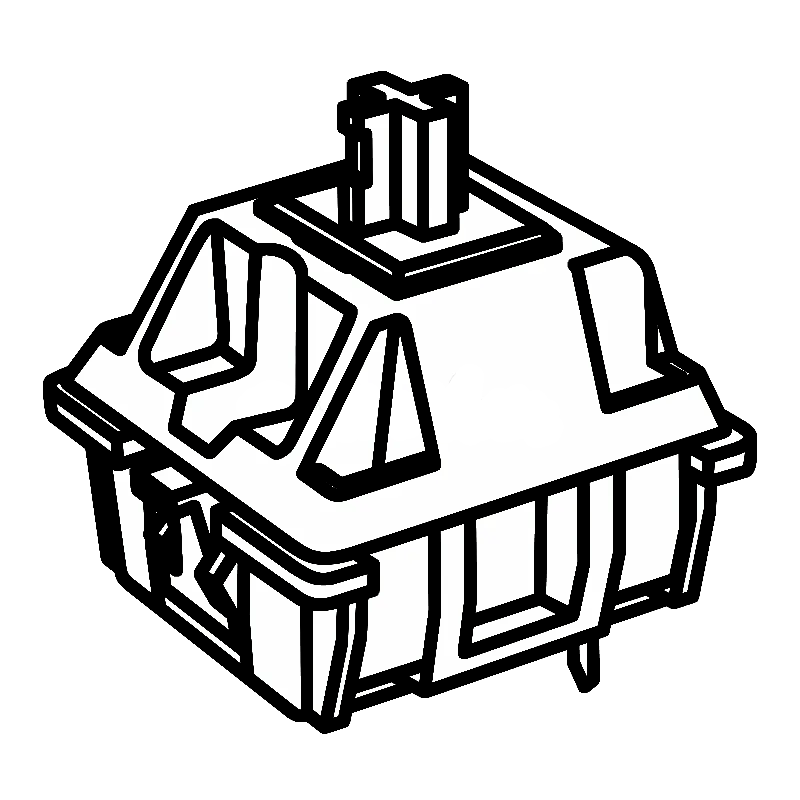
\includegraphics[width=0.8cm]{images/switch.png}
            } \\
            {\footnotesize Горные лыжи} & {\footnotesize Музыка} & {\footnotesize Гиперкубинг} & {\footnotesize Кастомные клавиатуры}
        \end{tabularx}
    }
}
\end{tabularx}
\end{center}
\end{document}
